%!TEX root = thesis.tex
% !TEX spellcheck = en-US
\chapter[Background]{Background}

\section{Energy efficiency} \label{energymeasurement}
Computers consume energy.
Achieving low energy consumption is an area of great interest, both in super computers where power is expensive, and in consumer hardware where low power mean longer battery life.
The energy consumption of a system depends both on hardware and software.
The hardware of the system will typically run within a narrow range of voltages, and the components of the system have some current draw when they are working.
The programmer can not affect how large these values are.
What can be done however, is to ensure that the software does not consume energy unnecessary.
Some of the components in the system that are not used, can be turned off.
Some of the features of a processor may also cause it to consume more power.
An example is NEON vector instructions, which have been shown to increase the power usage of the system by up to 20\% \cite{lillesand13} when used.
Turning off components or features does save power, but there will often be a performance loss.
When energy efficiency is a goal, there is always questions about how much power can be saved, before the execution time is extended so much that there is a total loss in energy consumed.
Because of this, it is interesting to analyze programs with regard to energy consumption.

\subsubsection{Energy measurement}
The interesting power properties of a system is voltage and current.
In systems featuring sensors for such data, the data can be gathered while executing a program.
By analyzing the data it is possible to optimize the program for energy efficiency.

The power of the system is the product of the voltage and current, as shown in Equation \ref{eq:powerconsumptionbackground}.
This is interesting to observe in applications that run when the system is standing by.
When execution time doesn't matter, the energy consumed per time becomes the only important metric.

\begin{equation} \label{eq:powerconsumptionbackground}
  Power = Current \times Voltage
\end{equation}

Often the system is executing a program for a duration, and as soon as it is done the system can be shut down.
In such cases it is interesting to measure how much energy the system consumed during execution.
The product of the systems power and the problems execution time, is as shown in Equation \ref{eq:energyconsumption} the total amount of energy consumed.

\begin{equation} \label{eq:energyconsumption}
  Energy\ consumption (Joule) = Power (Watt) \times Execution\ time (Second)
\end{equation}

There are many cases where a balance between energy efficiency and the performance trade off is interesting.
This is when the energy delay product of the system become interesting.
This is an interesting property for both scientific experiments and programs executed on regular systems.
In research experiments the goal may be to obtain energy efficiency or performance.
In either case, it is sensible to remember that the actual goal will normally be a balance between the two.
On regular systems in real life applications, both energy and performance matter.
Users do not want to wait longer than necessary for the system to complete its task.
Neither do they want the system to run out of battery, or the power bill to grow too big.
The energy delay product of a system is calculated by multiplying the execution time of the application with its energy, as shown in Equation \ref{eq:edp}.
\begin{equation} \label{eq:edp}
  Energy\ delay\ product = Energy \times Execution\ time
\end{equation}

\section{NEON}
NEON is a general-purpose single input multiple data (SIMD) technology implemented in the ARM Cortex-A series of processors.
It is able to run SIMD instructions on 128 bit registers.
By utilizing the NEON unit of the ARM processors, it is possible to achieve parallelism in each separate core.
This will often open for great performance boost on problems like the one explored in this paper.
Each register may be filled with single precision floating point numbers ranging from 8 to 64-bit each.
This mean that the programmer may choose to fill them with 16 8-bit numbers, 8 16-bit numbers, 4 32-bit numbers, 2 64-bit numbers or a single 128-bit number.
This allows a single thread to achieve parallelism.
In future generations of the ARM ISA there will be support for other data types as well \cite{neondata}.
Different implementations of NEON exist in the Cortex-A cores.
While the even the simple implementations in smaller cores like the Cortex-A7 can give great performance boost, the implementations present in the newest cores are performing even better.
The A15 offer two NEON units, and the instruction pipeline to start the cores are shorter than in simpler implementations.

\section{Task based programming}
Task based programming allow a programmer to work with parallel programs, with an abstraction from the parallelization itself.
When programming with this model, the program can be split into tasks which can run in parallel.
When the program run, it will run a task manager as part of the program.
This task manager can dynamically assign tasks to the processors, and the programmer does not have to handle all the time consuming tasks related to manual parallelization.
As long as the programmer correctly handle task dependencies in the parallelized code, it will be possible to write this kind of code as if it was serial.

The task based programming model also allow simpler development of portable programs.
When the program is running tasks on available CPUs, it is not a problem to allow it to run on larger or smaller numbers of processors, and even clusters can support the program.
This model even allow the tasks to run on different types of processors in a heterogeneous environment.

\section[OmpSs]{OpenMP Super scalar}
OpenMP Super scalar (OmpSs) is a extension of the OpenMP API to integrate features from the StarSs programming model.
It is currently under development at the Barcelona Supercomputing Center.
The goal of OmpSs is to extend the programming model to support a wide range of processors.
The OmpSs programming model run on a wide variety of different systems, such as traditional personal computers, clusters, shared memory systems and heterogeneous processors.
While the software is not yet completed or fully tested, there have been several reports exploring it's potential \cite{lillesand13}\cite{natvig12}.
The results have proven OmpSs as an efficient solution on a wide range of platforms.


\section{Heterogeneous multi-processor}
Heterogeneous multi-processor systems have multiple different processors, opposed to traditional multi-processor systems.
A typical modern processor have several processors, and a program can run effectively by having threads running parts of their work on each of them.
This work is often of such a nature that it can run better on a different processor.
Sometimes it can run just as well on multiple simple processor, while using less die space and energy.
In other instances, an advanced processor with some special capabilities, like vector instructions, can be more efficient.

This kind of processors have a potential to help us overcome the challenges that are emerging in processor development.
Unfortunately they also introduce several new challenges.
Both regular programs and operating systems can demand changes to be able to utilize such systems.

\section{ARM big.LITTLE} \label{bigLITTLE}

\section{Experiment platforms}

\subsection{Arndale Board} \label{ArndaleBoard}
\begin{figure}[ht!]
  \centering
  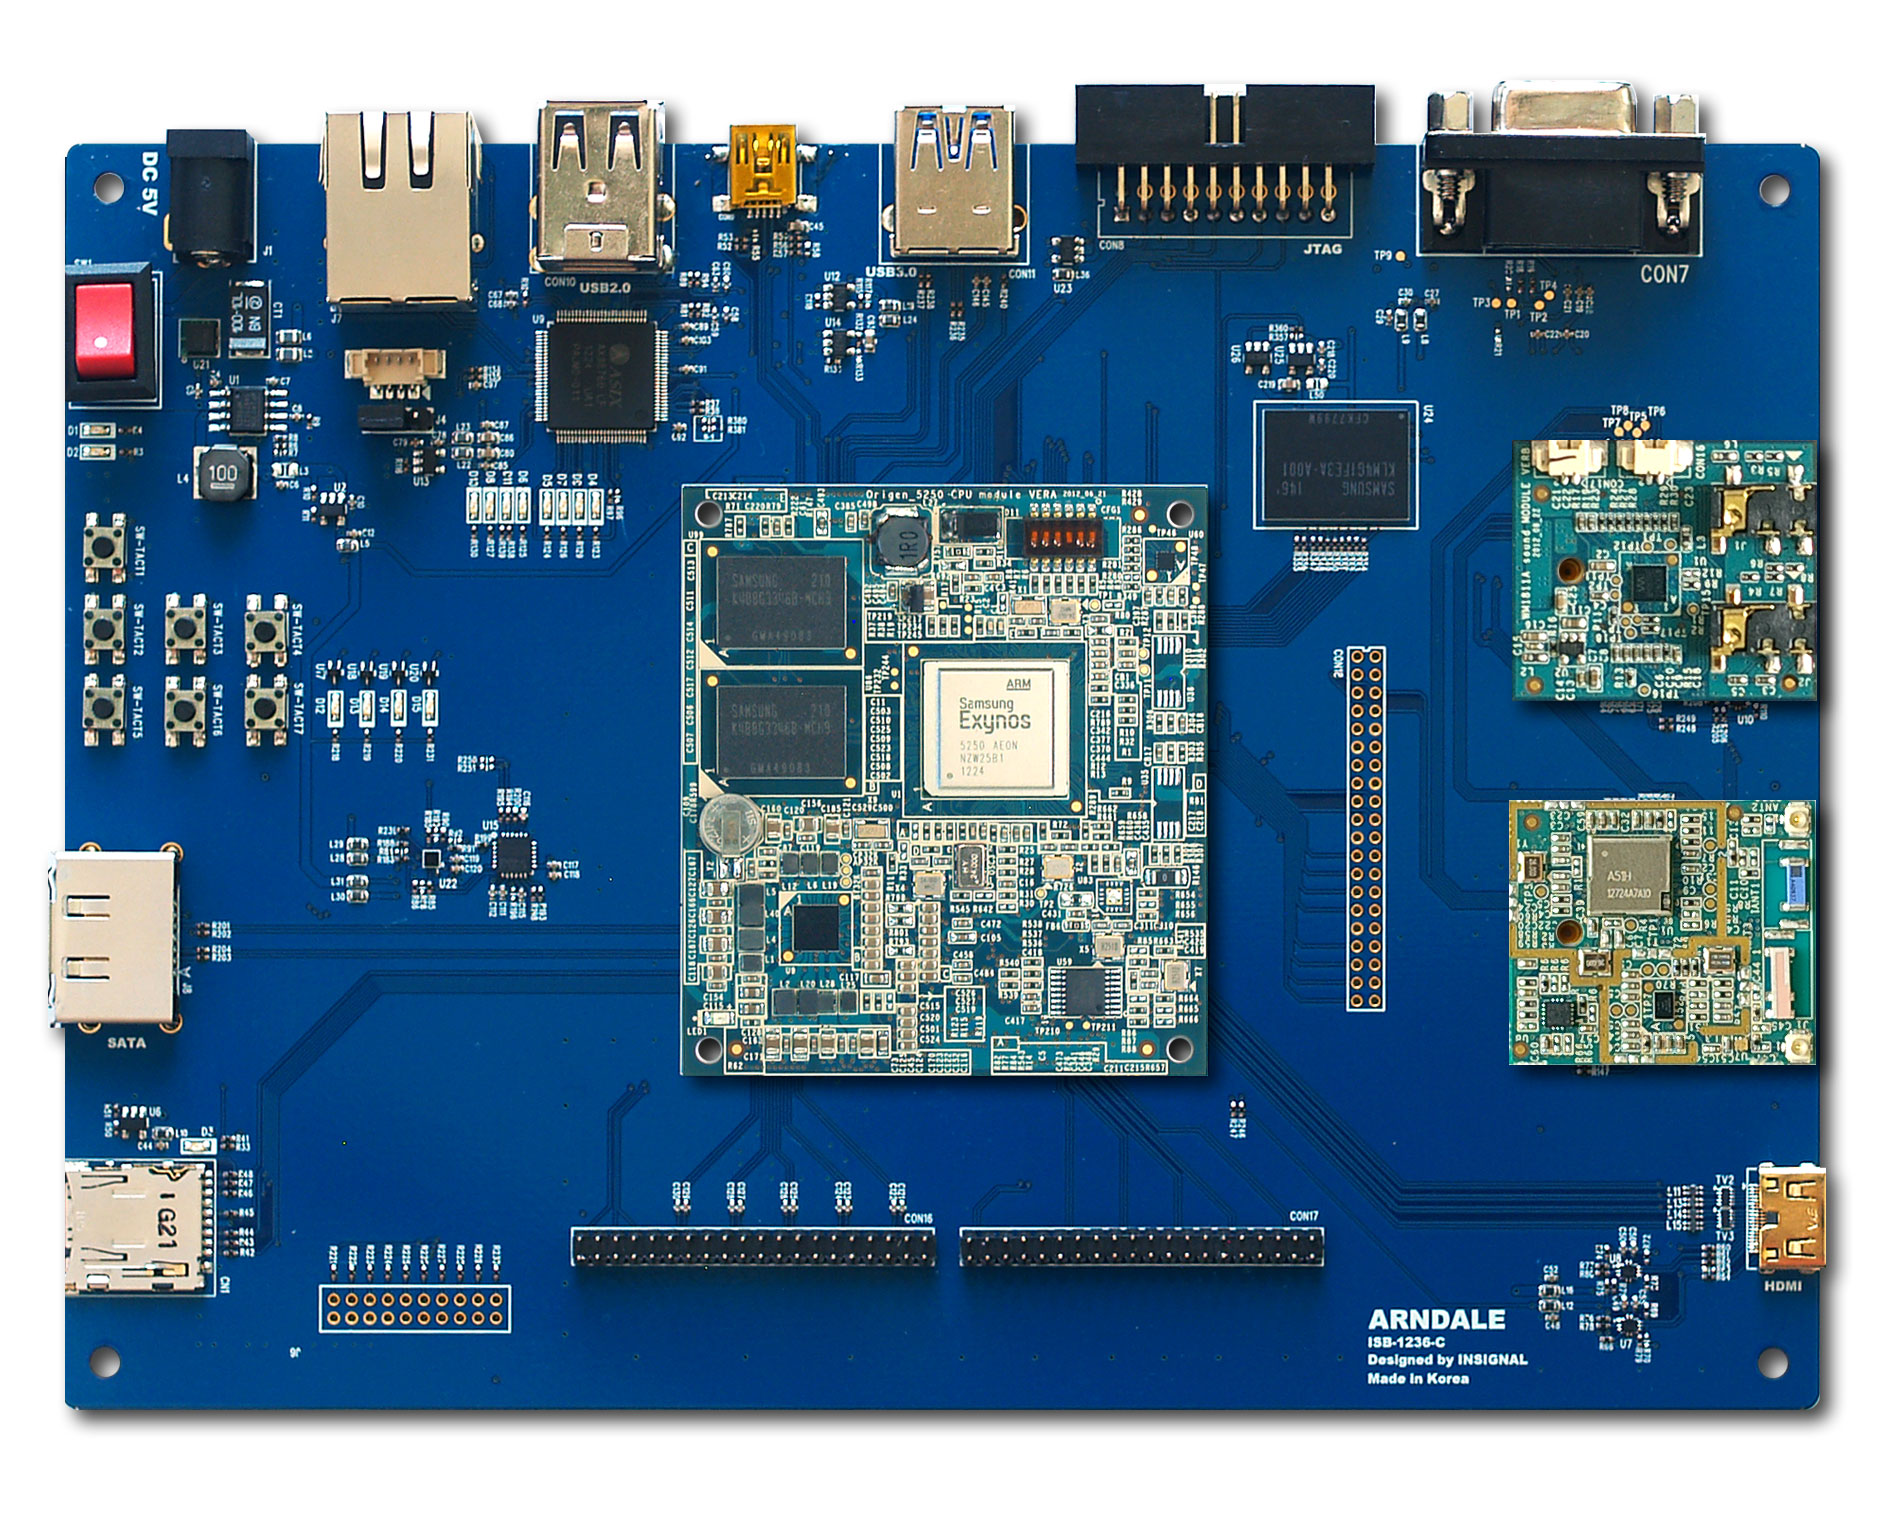
\includegraphics[width=90mm]{fig/Arendale.jpg}
  \caption{Arndale Board \label{ArndaleBoardImage}}
\end{figure}
The Arndale Board is the single board computing system shown in Figure \ref{ArndaleBoardImage}.
It is fitted with an Exynos 5250 SoC, which contain a dual core ARM Cortex-A15 , as well as an ARM Mali-T604 GPU.
This computer offer a range of supported Linux distributions, as well as the OmpSs programming model.
The Arndale Board was used for some preliminary research in this project.
It was chosen because we had experience from earlier student projects using this board.
The computer was used in the 2014 master thesis "Acceleration with OmpSs and Neon/OpenCL on ARM Processor" by Trond Inge Lillesand \cite{lillesand13}.
The thesis lay a lot of the foundation for this pilot project and planned master thesis.
In Table \ref{arndalespec} the system specifications of the board are listed.

\begin{table}[h]
  \centering
  \begin{tabular}{ll}
    \toprule
    \textbf{SoC}              & Samsung Exynos 5250 \\
    \midrule
    \textbf{CPU}              &  \\
    Model                     & ARM Cortex-A15 \\
    Manufacturing process     & 32nm \\
    Maximum clock frequency   & 1.7GHz \\
    Number of cores           & 2 \\
    L2 Cache                  & 1MB \\
    L1 Cache                  & 32KB \\
    \midrule
    \textbf{GPU}              &  \\
    Model                     & ARM Mali-T604 \\
    Maximum clock frequency   & 600 MHz \\
    \midrule
    \textbf{Memory}           &  \\
    Available memory          & 2 GB \\
    Maximum clock frequency   & 800MHz \\
    \midrule
    \textbf{Operating system} &  \\
    Distribution              & Linux Ubuntu \\
    %Version                   & TODO \\
    \bottomrule
  \end{tabular}
  \caption{Arndale Board specifications\label{arndalespec}}
\end{table}

\subsection{ODROID-XU3} \label{OdroidXU3}
\begin{figure}[H]
  \centering
  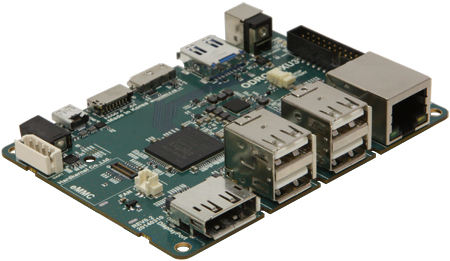
\includegraphics[width=90mm]{fig/ODROID.jpg}
  \caption{ODROID-XU3 \label{ODROIDImage}}
\end{figure}
The ODROID-XU3 is a new single-board computing system depicted in Figure \ref{ODROIDImage}, offering interesting properties for these experiments.
The system has an Exynos 5422 heterogeneous SoC.
Exynos 5422 has a quad core ARM Cortex-A15 CPU and a ARM Mali-T628 GPU, but also a smaller quad core ARM Cortex-A7 processor.
These 3 different processing units can be used simultaneously to solve problems.
They use ARMs big.LITTLE architecture, described in section \ref{bigLITTLE}, to achieve this heterogeneous cooperation.
In this paper, and the planned master thesis following it, the potency of this kind of heterogeneous processor will be explored.
This is the system that will run most of the experiments, including all energy efficiency experiments.
In Table \ref{ODROIDspec} the system specifications of the board are listed.

\begin{table}[H]
  \centering
  \begin{tabular}{ll}
    \toprule
    \textbf{SoC}              & Samsung Exynos 5422 \\
    \midrule
    \textbf{CPU 1}            &  \\
    Model                     & ARM Cortex-A15 \\
    Manufacturing process     & 32nm \\
    Maximum clock frequency   & 2.0GHz \\
    Number of cores           & 4 \\
    L2 Cache                  & 512KB \\
    L1 Cache                  & 32KB/32KB I/D \\
    \midrule
    \textbf{CPU 2}            &  \\
    Model                     & ARM Cortex-A7 \\
    Manufacturing process     & 32nm \\
    Maximum clock frequency   & 1.4GHz \\
    Number of cores           & 4 \\
    L2 Cache                  & 2MB \\
    L1 Cache                  & 32KB/32KB I/D \\
    \midrule
    \textbf{GPU}              &  \\
    Model                     & ARM Mali-T628 MP6 \\
    Maximum clock frequency   & 600 MHz \\
    \midrule
    \textbf{Memory}           &  \\
    Available memory          & 2 GB \\
    Maximum clock frequency   & 933MHz \\
    \midrule
    \textbf{Operating system} &  \\
    Distribution              & Linux odroid \\
    Version                   & 3.10.54+ \\
    \bottomrule
  \end{tabular}
  \caption{ODROID-XU3 specifications\label{ODROIDspec}}
\end{table}

\subsubsection{Power monitoring}
The ODROID-XU3 comes with integrated power monitoring tools.
Implemented in hardware, it has got 4 current sensors sitting on the power pins of the Exynos SoC.
The energy monitors are indicated in Figure \ref{overview-odroid}.
These monitor the current going through the large CPU cores, the small CPU cores, memory and GPU respectively.
In addition to the current sensors, the power management for the SoC is also available to the programmer, making supply voltage to the components known.
By using the voltage and current, the power consumption is known.
As a whole, the system offer frequency, voltage, current, temperature and power readings in real time.
These fine energy and performance metrics make the system highly suitable for developers.
They are able to run their programs, collect energy profiling data and optimize their software based on the result.

\begin{figure}[ht!]
  \centering
  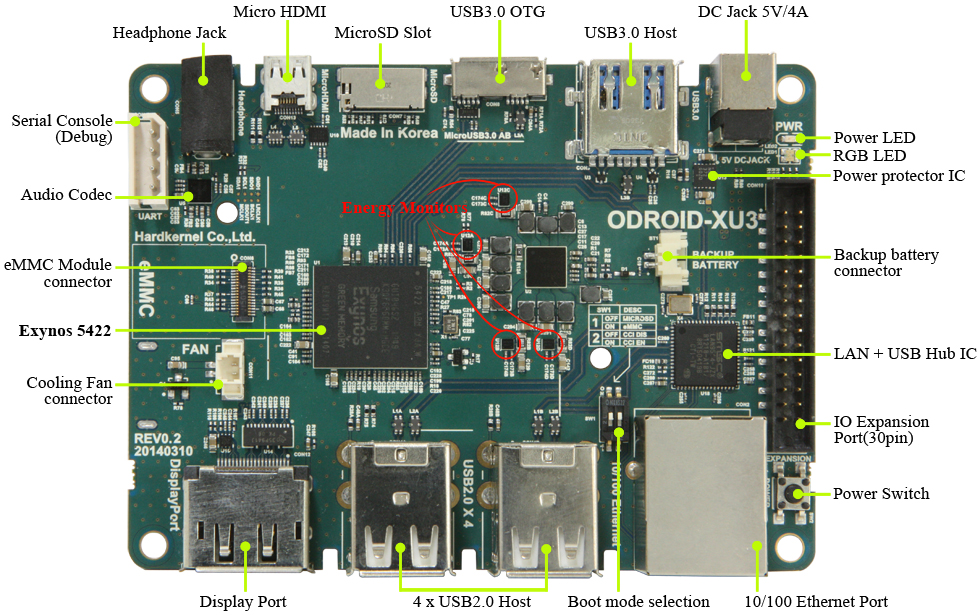
\includegraphics[width=130mm]{fig/overview-odroid.jpg}
  \caption{ODROID-XU3 annotated (hardkernel.com\cite{hardkernel01})\label{overview-odroid}}
\end{figure}

\subsubsection{Performance}

The ODROID-XU3 comes with the ARM Cortex-A15 limited to 2GHz and the ARM Cortex-A7 limited to 1.4GHz.
There is 2GB of memory available running at 800 MHz, and the ARM Mali-T628 GPU run at 600 MHz.
This performance place it at the higher end of SoCs, but not quite in the top, as it is beaten by systems like TODO A reference system here).
The ODROID-XU3 feature the new eMMC 5.0 standard for storage.
The performance of this standard outperform both older eMMC standards, as well as memory card readers, which other similar systems may contain.
The ODROID-XU3 can achieve a read/write performance of 198/74 MB/s\cite{hardkernel01}, which a lot better than older systems like the Arndale Board.

In addition to the eight processor cores, the system also feature a ARM Mali-T628.
The Mali-T628 function both as a regular GPU, as well as a GPGPU.
It support both OpenGL and DirectX, and is able to produce graphics for all but the most demanding gaming and simulation purposes.
In addition to this it is able to run computations with OpenCL.
This mean that problems with parallel parts, can be solved efficiently utilizing the GPU.

\subsection{ARM Cortex-A15}
The ARM Cortex-A15 is a high performance processor core designed for use in a wide range of applications, from small embedded systems, to larger consumer electronics.
The specifications of the core are listed in Table \ref{A15}.
This processor core is present in both the Arndale Board and the ODROID-XU3, who have 2 and 4 such cores respectively.
In the latter, 4 smaller ARM Cortex-A7 cores are also featured, and all can be used simultaneously.
\begin{table}[H]
  \centering
  \begin{tabular}{ll}
    \toprule
    Frequency         & 1.0 GHz to 2.5GHz  \\
    \midrule
    L1 Cache          & 64KB \\
    L2 Cache          & 4 MB \\
    L3 Cache          & None in core, may be implemented shared in multi core system. \\Architecture      & ARMv7-A            \\
    \midrule
    Architecture      & ARMv7-A            \\
    \midrule
    Supported features& TrustZone® security technology \\
                      & NEON™ Advanced SIMD \\
                      & DSP \& SIMD extensions \\
                      & VFPv4 Floating point \\
                      & Hardware vitalization support \\
                      & Integer Divide \\
                      & Fused MAC \\
                      & Hypervisor debug instructions \\
    \midrule
    Memory management & 40-bit ARMv7 Memory Management Unit \\
    \bottomrule
  \end{tabular}
  \caption{ARM Cortex-A15 specifications\label{A15}}
\end{table}
\subsection{ARM Cortex-A7}
The ARM Cortex-A7 is designed to be a low power alternative to the ARM Cortex-A15 and ARM Cortex-A17, with the same supported ISA and features.
The specifications of the core are listed in Table \ref{A7}.
This enable the ARM Cortex-A7 to be paired with it's larger relatives in a ARM big.LITTLE configuration.
The Exynos 5422 SoC on the ODROID-XU3 board feature 4 of these cores.
\begin{table}[H]
  \centering
  \begin{tabular}{ll}
    \toprule
    Frequency         & 1.2 GHz to 1.6GHz  \\
    \midrule
    L1 Cache          & 8-64KB \\
    L2 Cache          & up to 1 MB \\
    L3 Cache          & None in core, may be implemented shared in multi core system. \\
    \midrule
    Architecture      & ARMv7-A            \\
    \midrule
    Supported features& ARM Thumb-2 \\
                      & TrustZone® security technology \\
                      & NEON™ Advanced SIMD \\
                      & DSP \& SIMD extensions \\
                      & VFPv4 Floating point \\
                      & Hardware vitalization support \\
                      & Integer Divide \\
                      & Fused MAC \\
                      & Hypervisor debug instructions \\
    \midrule
    Memory management & 40-bit ARMv7 Memory Management Unit \\
    \bottomrule
  \end{tabular}
  \caption{ARM Cortex-A7 specifications\label{A7}}
\end{table}
\subsection{ARM Mali-T604}
This is a high performance low power mobile GPU.
The specifications of the GPU are listed in Table \ref{T604}.
The Arndale Board feature one of these in it's Exynos 5250 SoC.
\begin{table}[H]
  \centering
  \begin{tabular}{ll}
    \toprule
    Frequency         & 533 MHz\\
                      & 17 GFLOPS  \\
    \midrule
    Multi core support & 1-4 cores  \\
    \midrule
    API Support       & OpenGL 1.1, 2.0, 3.0 and 3.1  \\
                      & OpenCL 1.1  \\
                      & DirectX 11  \\
                      & RenderScript \\
    \midrule
    Anti-Aliasing     & 4xFSAA with minimal performance drop  \\
                      & 16xFSAA  \\
    \midrule
    Cache             & 32-256KB L2 cache \\
    \bottomrule
  \end{tabular}
  \caption{ARM Mali-T604 specifications\label{T604}}
\end{table}

\subsection{ARM Mali-T628}
This is a high performance low power mobile GPU.
The specifications of the GPU are listed in Table \ref{T628}.
The ODROID-XU3 board feature one of these in it's Exynos 5244 SoC.
\begin{table}[H]
  \centering
  \begin{tabular}{ll}
    \toprule
    Frequency         & 533/695 MHz \\
                      & 17/23.7 GFLOPS \\
    \midrule
    Multi core support & 1-8 cores  \\
    \midrule
    API Support       & OpenGL 1.1, 2.0, 3.0 and 3.1  \\
                      & OpenCL 1.1  \\
                      & DirectX 11  \\
                      & RenderScript \\
    \midrule
    Anti-Aliasing     & 4xFSAA with minimal performance drop  \\
                      & 16xFSAA  \\
    \midrule
    Cache             & 32-256KB L2 cache \\
    \bottomrule
  \end{tabular}
  \caption{ARM Mali-T628 specifications\label{T628}}
\end{table}

\section{2D-Convolution}
Convolution is a mathematical operation to combine two functions into a third output function.
The resulting output function maintain properties from both the input functions.
It is useful in a wide range of problems within mathematics, statistics, electrical engineering and computer science.
An example is computer vision, which can use convolutions to filter data.
Use an image as the first input and a sobel filter as the second.
The output would then be an image with all emphasized.

2D-Convolution on discrete input data will have an output with each pixel [m,n] defined as \cite{lillesand13}:

\begin{equation} \label{eq:2dconvolutionpixel}
  y[m,n] = x[m,n] \times h[m,n] = \sum\limits_{j=-\infty}^\infty \sum\limits_{i=-\infty}^\infty input[i,j] \times filter[1-i, 1-j]
\end{equation}

The limits are in reality smaller than $\infty$ as they can be set to the size of the input image and filter.
2D-Convolution is convenient for this paper, as each pixel of the output is independent.
This computation for each pixel or small group of pixels can made a task in OmpSs.

In the implementation of 2D-Convolution used in this project, Equation \ref{eq:2dconvolutionpixel} is run for each pixel in the input image.
The limits are set to the size of the input.
This result Equation \ref{eq:2dconvolution} \cite{lillesand13}.

\begin{equation} \label{eq:2dconvolution}
  Y = X \times H = \sum\limits_{m=0}^W \sum\limits_{n=0}^H \sum\limits_{j=0}^{w} \sum\limits_{i=0}^{h} input[i,j] \times filter[1-i, 1-j]
\end{equation}

The 4 loops in Equation \ref{eq:2dconvolution} show that the number of operations in this problem is $W\times H\times w\times h$.
This is a time complexity of $\mathcal{O}(n^4)$ when W=H=w=h \cite{burger09}.

